\chapter{Marco Metodológico}
Determinación de la población de estudio, la cual debe contar con características similares, como, por ejemplo: diestros, del mismo sexo, en un rango de edad de seis años. Un estudio con un número de participantes mayor a veintidós puede aportar mejores resultados (Davatzikos et al., 2005). Sobre la población de estudio, se conducen las pruebas para determinar el engaño. 

Utilización de un método para conducir al engaño en la población de estudio, como, por ejemplo, un juego con cartas con instrucciones contradictorias, en donde se maneje dinero (Davatzikos et al., 2005). De igual manera, puede manejarse una prueba en donde se motive a los sujetos de prueba a decir la verdad, o a decir una mentira sin ser detectados por los investigadores, involucrando de igual manera dinero para aumentar dicha motivación y ansiedad (Revell et al., 2004). Una prueba con características similares se efectúa con los individuos de estudio. Durante este proceso, se obtiene información del dispositivo Emotiv, en donde se leen las señales electroencefalográficas. 

Análisis de los datos para poder ser clasificados. Utilizar statistical parametric mapping para procesar y analizar datos funcionales. Corregir los tiempos de las imágenes, normalizar las pruebas e interpolarlas. Suavizar las imágenes con métodos gaussianos (Davatzikos et al., 2005). De esta manera, se obtiene información estandarizada para los algoritmos a utilizar. Este proceso de análisis de los datos se encuentra luego de obtener los datos de los individuos, y antes de ser clasificados por los algoritmos a utilizar. De estos datos obtenidos, se utilizará más del cincuenta por ciento para entrenar al algoritmo. El resto se utilizarán para la validación de datos. 

Utilizar Support Vector Machine no lineal para clasificar los datos. En pruebas similares, con veintidós participantes, se analizaron 560 variables, con 1056 imágenes de estimación de parámetros de pruebas (Davatzikos et al., 2005). Se espera analizar un valor igual o mayor de variables con este algoritmo, dado el mayor número de participantes.

Determinar el valor de efectividad de detección del engaño de este algoritmo, a partir de los datos obtenidos en la prueba realizada reservados para la validación del algoritmo. Esto consistirá en medir la cantidad de aciertos que el algoritmo tenga cuando se busque predecir el resultado de los participantes. Ya que efectivamente se posee la respuesta de estos, se puede obtener un valor de aciertos del algoritmo con respecto al valor real estudiado.   

\begin{center}
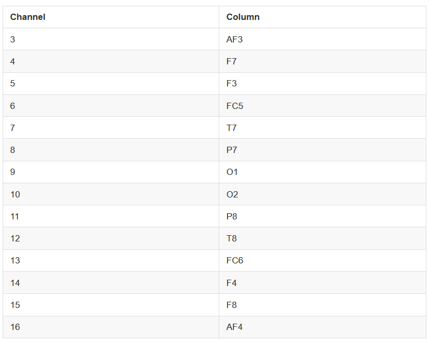
\includegraphics[height=2.15in]{figuras/Imagen4.png}
\end{center}

\begin{center}
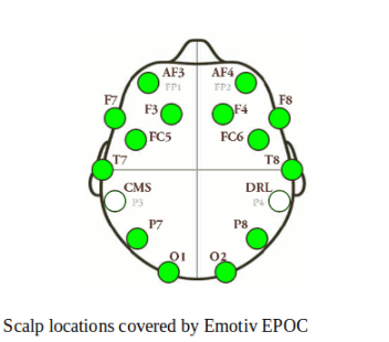
\includegraphics[height=2.15in]{figuras/Imagen3.png}
\end{center}

\begin{center}
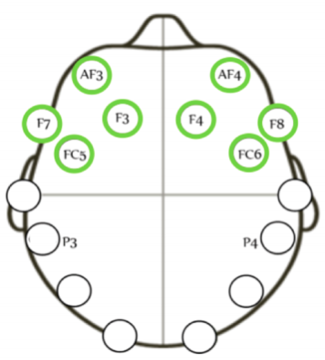
\includegraphics[height=2.15in]{figuras/Imagen2.png}
\end{center}




\chapter{Resultados}

\begin{center}
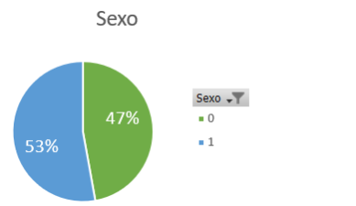
\includegraphics[height=1.15in]{figuras/Imagen11.png}
\end{center}

\begin{center}
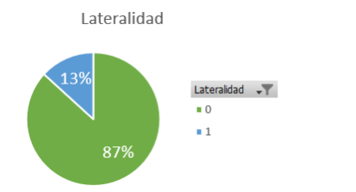
\includegraphics[height=1.15in]{figuras/Imagen12.png}
\end{center}

\begin{center}
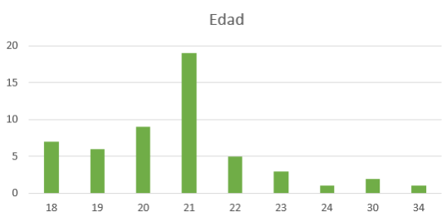
\includegraphics[height=1.15in]{figuras/Imagen13.png}
\end{center}

\begin{center}
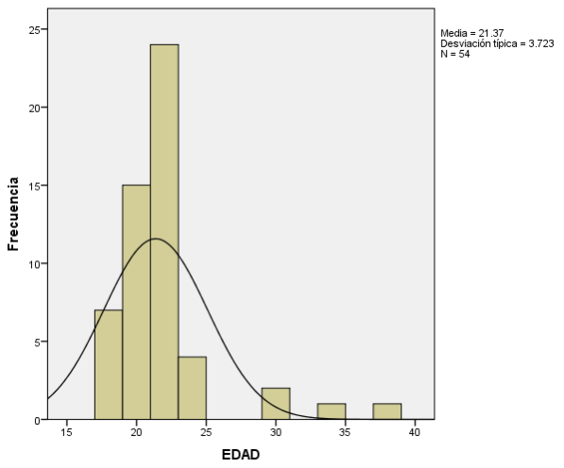
\includegraphics[height=1.15in]{figuras/Imagen14.png}
\end{center}

\begin{center}
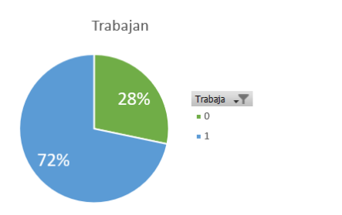
\includegraphics[height=1.15in]{figuras/Imagen15.png}
\end{center}

\begin{center}
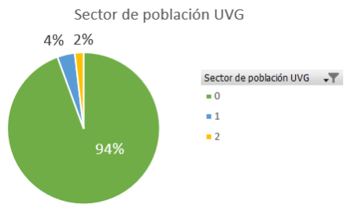
\includegraphics[height=1.15in]{figuras/Imagen16.png}
\end{center}

\begin{center}
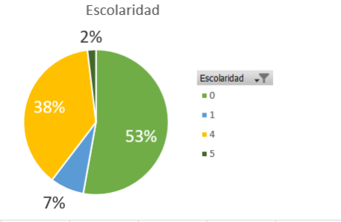
\includegraphics[height=1.15in]{figuras/Imagen17.png}
\end{center}

\begin{center}
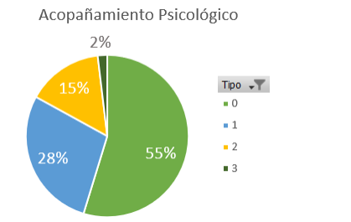
\includegraphics[height=1.15in]{figuras/Imagen18.png}
\end{center}

\begin{center}
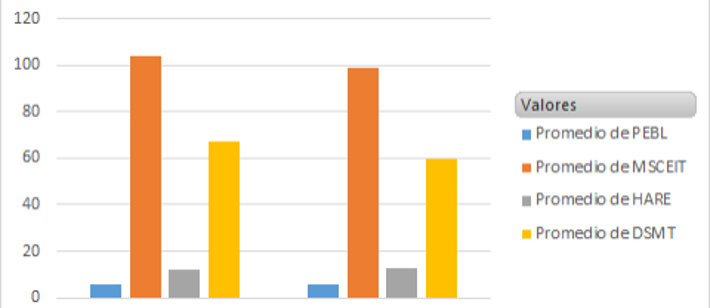
\includegraphics[height=1.15in]{figuras/Imagen19.png}
\end{center}

\begin{center}
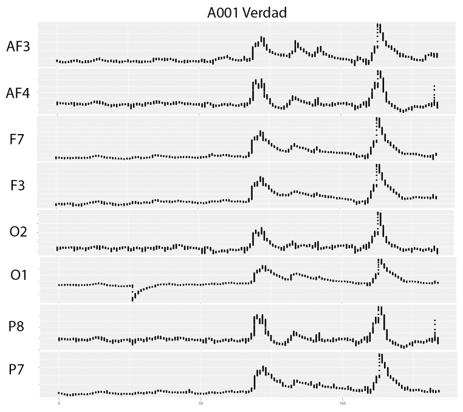
\includegraphics[height=3.0in]{figuras/Imagen5.png}
\end{center}

\begin{center}
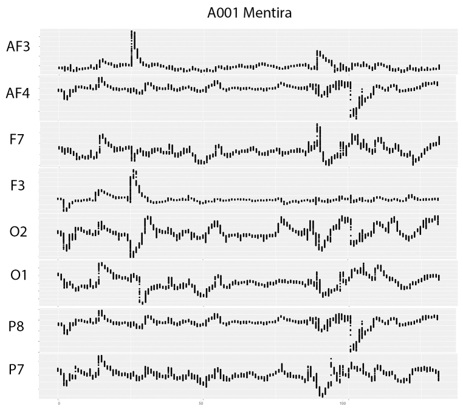
\includegraphics[height=3.0in]{figuras/Imagen6.png}
\end{center}

\begin{center}
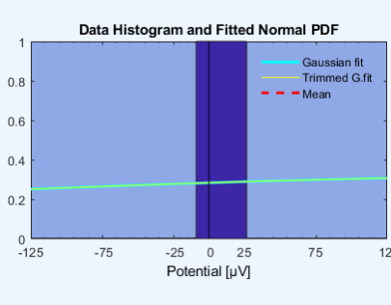
\includegraphics[height=2.35in]{figuras/Imagen7.png}
\end{center}

\begin{center}
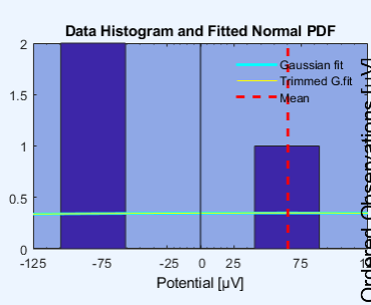
\includegraphics[height=2.35in]{figuras/Imagen8.png}
\end{center}

\begin{center}
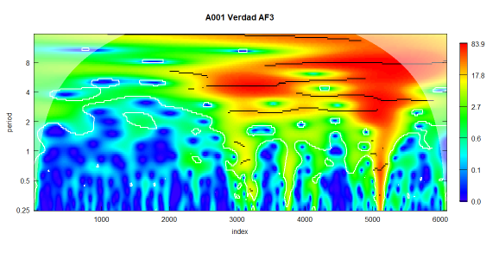
\includegraphics[height=3.0in]{figuras/Imagen9.png}
\end{center}

\begin{center}
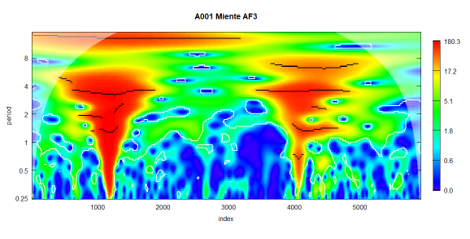
\includegraphics[height=3.0in]{figuras/Imagen10.png}
\end{center}

\begin{center}
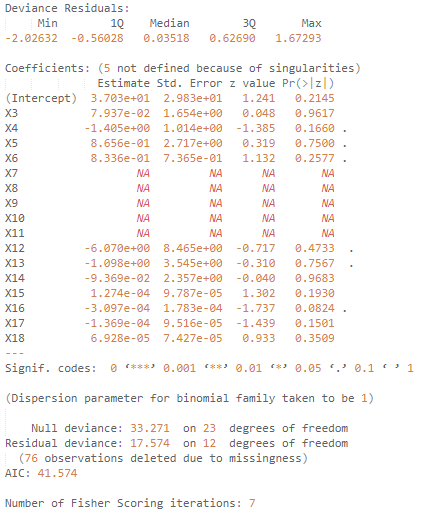
\includegraphics[height=3.3in]{figuras/Capture4.PNG}
\end{center}

\begin{center}
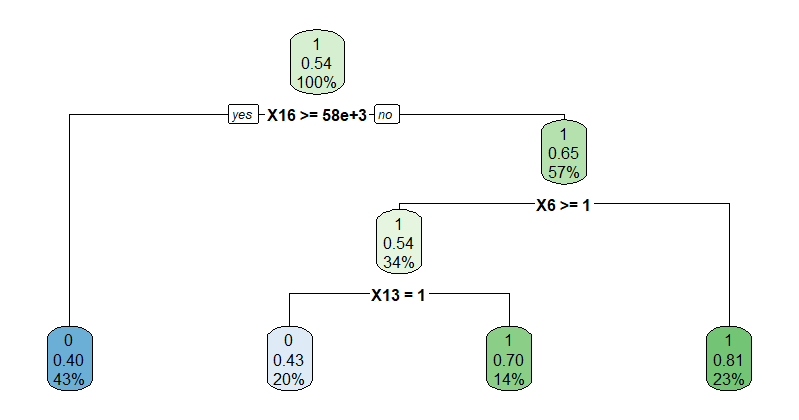
\includegraphics[height=3.0in]{figuras/Rplot1.png}
\end{center}

\begin{center}
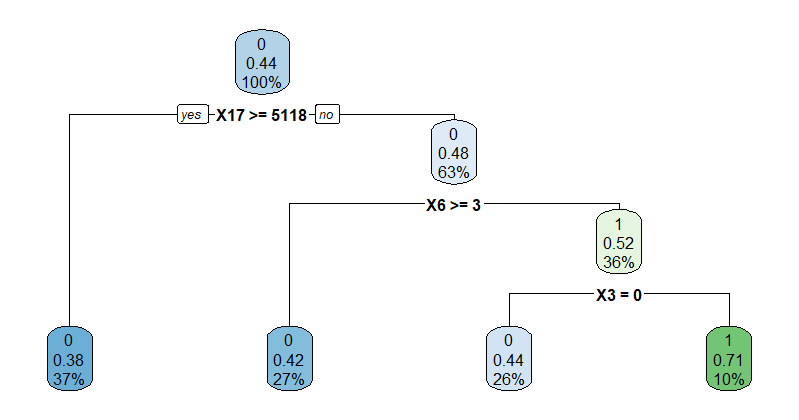
\includegraphics[height=3.0in]{figuras/Rplot2.png}
\end{center}

\begin{center}
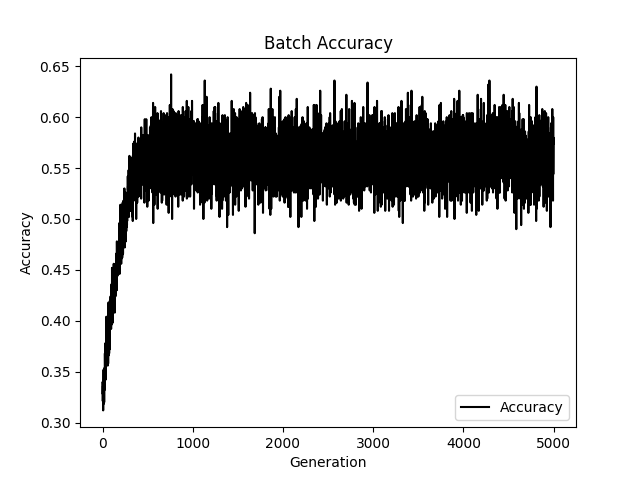
\includegraphics[height=3.0in]{figuras/Figure_1.png}
\end{center}

\begin{center}
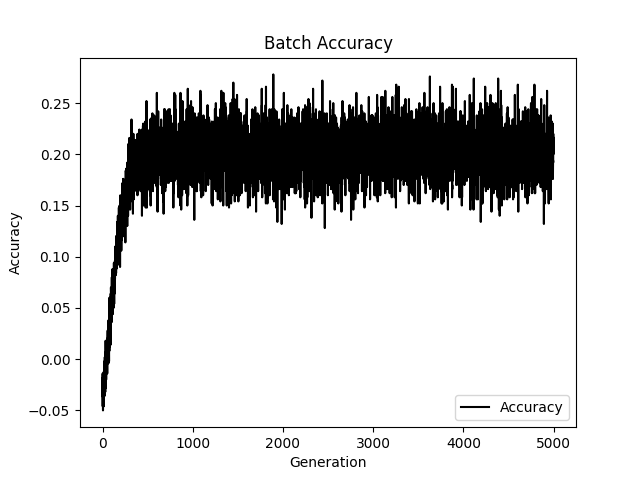
\includegraphics[height=3.0in]{figuras/Figure_2.png}
\end{center}

\begin{center}
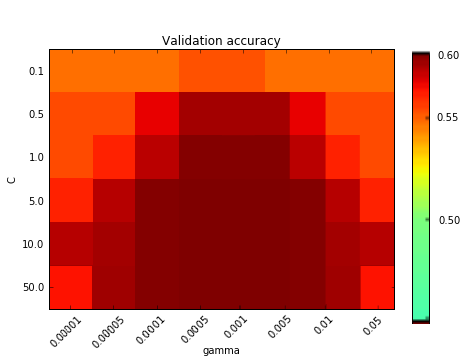
\includegraphics[height=3.0in]{figuras/58e171451b12ce00012bd71d.png}
\end{center}

\begin{center}
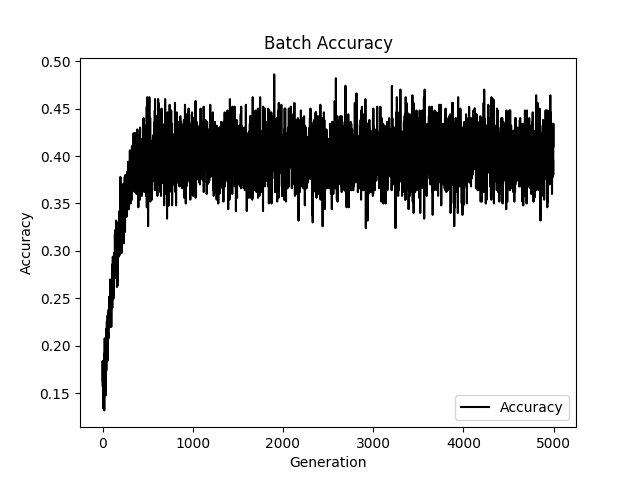
\includegraphics[height=3.0in]{figuras/Figure_3.png}
\end{center}

\begin{center}
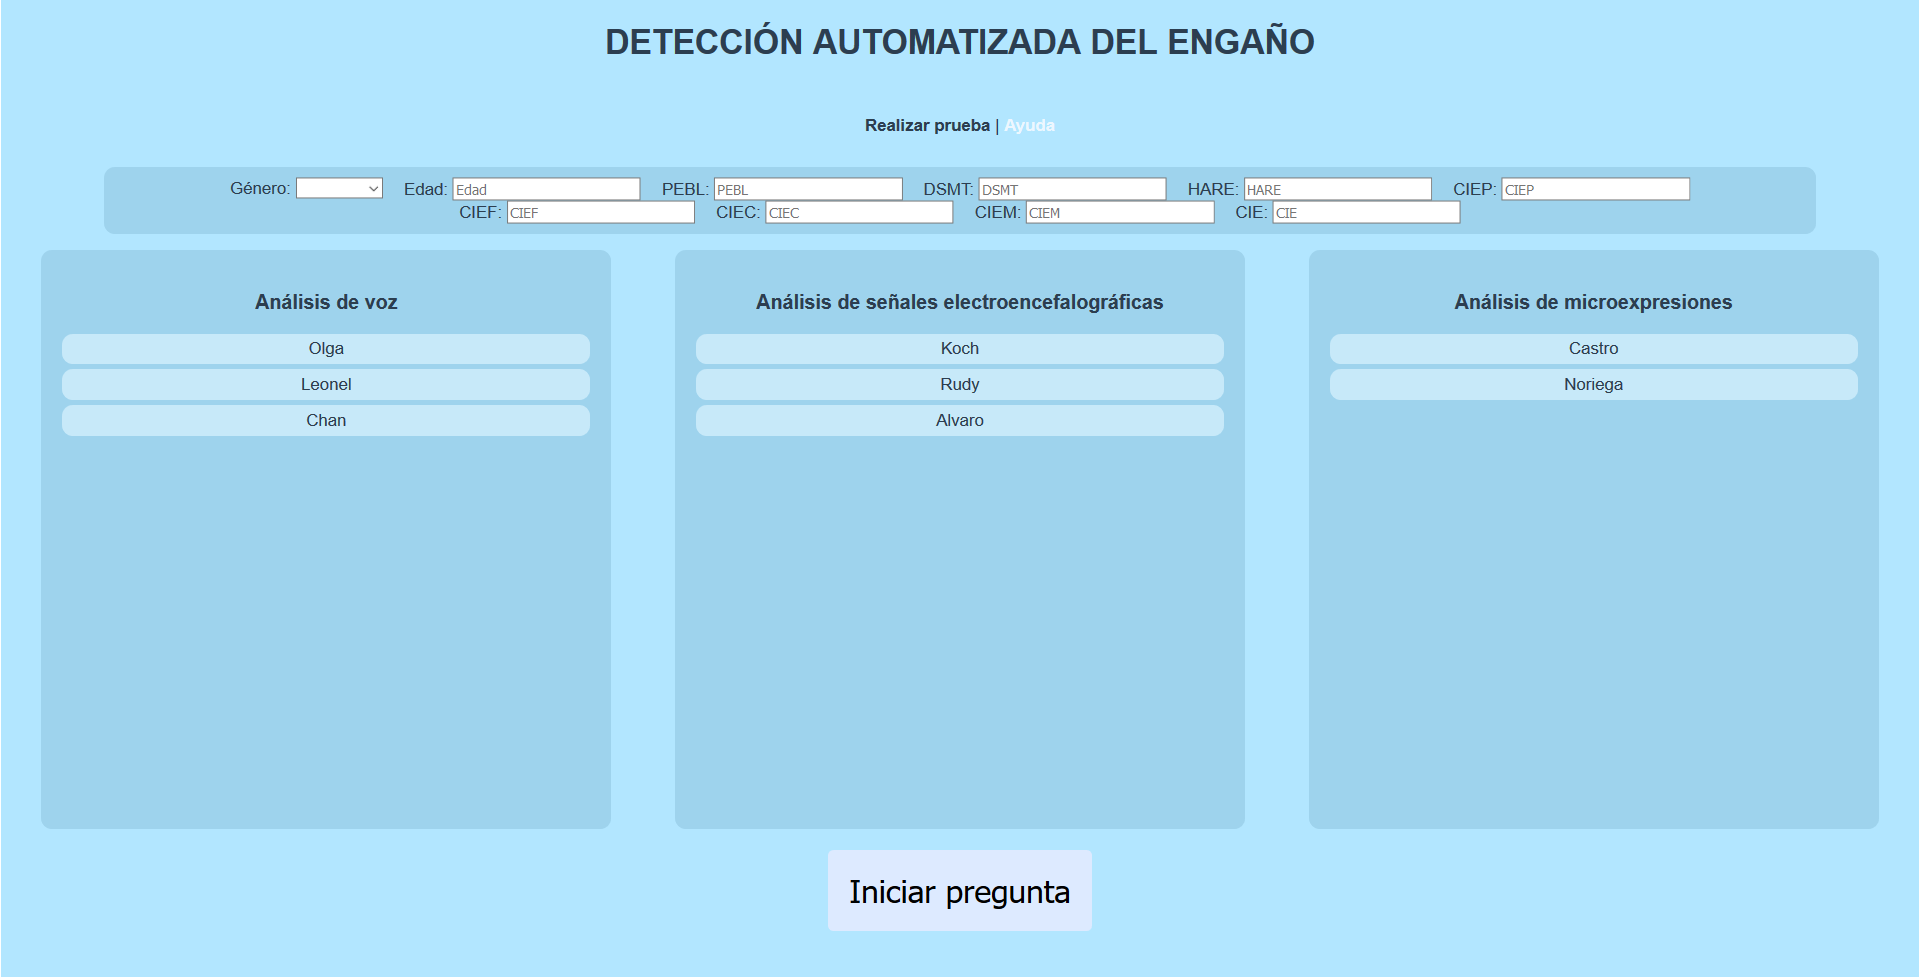
\includegraphics[height=3.15in]{figuras/Imagen20.PNG}
\end{center}



\chapter{Análisis de Resultados}
%\section{Dinámica de cuerpos rígidos}
%\section{Restricciones}
%\subsection{Mecanismos de lazo cerrado}
%\subsubsection{Mecanismo de cuatro barras}
%\chapter{Control del sistema mecánico}
%\section{La ecuación del manipulador}